\documentclass{article}
\usepackage[utf8]{inputenc}
\usepackage{setspace}
\usepackage[export]{adjustbox}
\renewcommand{\thefigure}{\arabic{section}.\arabic{figure}}
\usepackage{amsmath}
\usepackage{amssymb}
\usepackage{graphicx}
\usepackage{apacite}
\usepackage{acronym} 
\usepackage{tabularx}
\usepackage{array}
\usepackage{sectsty}

% Instructions
% Add internal and external 
% Change the approval part and convert it into like 3rd person approving it.
% Add summary section in each section

%%%%%%%%%% added
% \usepackage{booktabs}
% \usepackage{multirow}
% \usepackage{cite}


% IEEE bibliography using biblatex
\usepackage[
    backend=biber,
    style=ieee,
    sorting=none,
    maxbibnames=99,
    maxcitenames=99,
    giveninits=true,
    doi=true,
    isbn=false,
    url=true,
    eprint=false
]{biblatex}

\addbibresource{ref.bib}

%\usepackage{biblatex} %Imports biblatex package

%\addbibresource{ref.bib} %Import the bibliography file
%%%%%%%%%%%%%%%%

\sectionfont{\fontsize{16}{16}\selectfont}
\subsectionfont{\fontsize{14}{14}\selectfont}
\subsubsectionfont{\fontsize{14}{14}\selectfont}
\paragraphfont{\fontsize{12}{12}\selectfont}
\subparagraphfont{\fontsize{12}{12}\selectfont}


\usepackage{hyperref}
\hypersetup{
    colorlinks,
    citecolor=black,
    filecolor=black,
    linkcolor=black,
    urlcolor=black
}

\usepackage[a4paper,left=3cm,right=3cm,top=3cm,bottom=2.5cm]{geometry}
\begin{document}
\doublespacing

\begin{titlepage}
% % The paper headers and footers
% \thispagestyle{fancyplain}
% \fancyhf{}
% \lhead{\fancyplain{}{Version 1.0}}
% \renewcommand{\headrulewidth}{0pt}
    \begin{center}
    \hrule
    \vspace{4mm}
     \large \textbf{Title of the Thesis/Report}
    \vspace{4mm}
    \hrule 
    \vspace{18mm}
    By\\
    1st group member name \hspace{15mm} ID: .......... \\
    2nd group member name \hspace{14mm} ID: .......... \\
    3rd group member name \hspace{15mm} ID: .......... \\
    4th group member name \hspace{15mm} ID: .......... \\
    5th group member name \hspace{15mm} ID: .......... \\
    \vspace{5mm}
    \textbf{Supervisor}\\
    Sudipto Chaki\\
    Assistant Professor, CSE, BUBT\\
    \vspace{5mm}
    \large Submitted in partial fulfillment of the requirements of the degree of\\
\large  \textbf{Bachelor of Science in} \\
\large \textbf{Computer Science and Engineering}\\
\vspace{10mm}

\includegraphics[scale=0.25]{image/BUBT-Logo.png}

\large Department of Computer Science and Engineering\\
\large Bangladesh University of Business and Technology\\
\vspace{10mm}
\large July 2026
    
    \end{center}
\end{titlepage}

% \tableofcontents
% \thispagestyle{empty}
% \cleardoublepage 
\pagenumbering{roman}
\setcounter{page}{2}

\begin{center}
    \section*{Declaration}
\end{center}
\large 


We do hereby declare that the research works presented in this thesis entitled, “Thesis/Report Title” are the results of our works. We further declare that the thesis/report has been compiled and written by us, and no part of this thesis/report has been submitted elsewhere for the requirements of any degree, award, diploma, or any other purposes except for publications. The materials that are obtained from other sources are duly acknowledged in this thesis.


\vspace{10mm}
\begin{flushleft}

\textbf{\underline{Signature of Authors}} \null\hfill  

\vspace{10mm}

\underline{
\includegraphics[scale=0.7]{image/khaled.png}} \null\hfill 
\underline{
\includegraphics[scale=0.4]{image/khaled.png}}\\
1st group member name \null\hfill   2nd group member name \\
ID: ..........  \null\hfill  ID: .......... \\

\vspace{5mm}

\underline{
\includegraphics[scale=0.4]{image/khaled.png}} \null\hfill 
\underline{
\includegraphics[scale=0.7]{image/khaled.png}}\\
3rd group member name  \null\hfill   4th group member name\\
ID: ..........  \null\hfill  ID: ..........\\

\vspace{5mm}

\underline{
\includegraphics[scale=0.5]{image/khaled.png}}\\
5th group member name\\
ID: .......... \\ 
\end{flushleft}
\addcontentsline{toc}{section}{Declaration}
\cleardoublepage

\begin{center}
    \section*{Approval}
\end{center}

\noindent
It is hereby certified that the research work presented in this thesis entitled, “Thesis/Report Title,” is the result of the original work carried out by 1st Group Member Name, 2nd Group Member Name, 3rd Group Member Name, 4th Group Member Name, and 5th Group Member Name. Furthermore, it is certified that this thesis/report satisfies the requirements and standards for the degree of Bachelor of Science in Computer Science and Engineering.


\vspace{10mm}


\begin{table}[!h]
\centering
\renewcommand{\arraystretch}{1.7}

\begin{tabular*}{\textwidth}{@{\extracolsep{\fill}} p{0.55\textwidth} >{\raggedleft\arraybackslash}p{0.35\textwidth}}

\underline{\hspace{6cm}} &
\\[-0.1cm]
\textbf{Md. Mamun Hossain} &
\textbf{Supervisor} \\
Assistant Professor, CSE &
Capstone Defense Board \\
BUBT, Dhaka-1216 &
\\[0.8cm]

\underline{\hspace{6cm}} &
\\[-0.1cm]
\textbf{Sudipto Chaki} &
\textbf{Member (Internal)} \\
Assistant Professor, CSE &
Capstone Defense Board \\
BUBT, Dhaka-1216 &
\\[0.8cm]

\underline{\hspace{6cm}} &
\\[-0.1cm]
\textbf{Dr. M. Shamim Kaiser} &
\textbf{Member (External)} \\
Professor, IIT &
Capstone Defense Board \\
JU, Savar-1342 &
\\[0.8cm]

\underline{\hspace{6cm}} &
\\[-0.1cm]
\textbf{Prof. Dr. Md. Ahsan Habib} &
\textbf{Convener} \\
Chairman, CSE &
Capstone Defense Board \\
BUBT, Dhaka-1216 &
\\[1cm]

\multicolumn{2}{c}{\textbf{Department of Computer Science and Engineering, BUBT, Dhaka.}}\\
\end{tabular*}
\end{table}


\addcontentsline{toc}{section}{Approval}
\cleardoublepage



\begin{center}
    \section*{Dedication}
\end{center}
\large We dedicate this research to our loving parents, whose unwavering love,
    encouragement, sacrifices, and constant support have been the foundation
    of our academic journey. Their guidance and belief in our abilities have
    inspired us to overcome challenges and pursue excellence. This work is
    also dedicated to our families, teachers, and well-wishers for their
    continuous motivation and encouragement throughout the completion of this
    thesis.
\addcontentsline{toc}{section}{Dedication}
\cleardoublepage

\begin{center}
    \section*{Acknowledgement}
\end{center}
\large We would like to express our heartfelt gratitude to the almighty Allah who offered our family and us kind care throughout this journey. We are deeply thankful to the Bangladesh University of Business and Technology (BUBT) for providing us with such a wonderful environment to pursue our research/project. We would like to express our sincere gratitude to Supervisor Name, Designation, Department of CSE, BUBT. We have completed our research with his/her help. We found the research area, topic, and problem with his/her suggestions. He/She guided us with our study and supplied us with many research papers and academic resources in this area. He/She is patient and responsible. When we had questions and needed his/her help, he/she would always find time to meet and discuss with us no matter how busy he/she was. We also want to give thanks to Chairman Name, Designation, Department of CSE, and all our teachers for providing a solid background for our studies and research thereafter. They have been a great source of inspiration to us, and we thank them from the bottom of our hearts. We would also like to acknowledge our team members for supporting each other and be grateful to our university for providing this opportunity for us.
\addcontentsline{toc}{section}{Acknowledgement}
\cleardoublepage

\begin{center}
    \section*{Abstract}
\end{center}
Early and accurate detection of lung and colon cancer is critical for improving patient survival rates. However, conventional classification techniques often struggle with the complexity of medical imaging data. In this study, we propose a novel hybrid architecture, the Separable Convolution and Attention Mechanism (SCA-mechanism), to enhance the accuracy of cancer classification. The proposed model integrates separable convolutions with residual connections to facilitate efficient feature extraction while incorporating attention mechanisms to emphasize key regions indicative of malignancy. We evaluated the performance of the SCA-mechanism model against state-of-the-art deep learning techniques using a benchmark dataset of lung and colon cancer images. Experimental results demonstrate that our proposed approach achieves superior classification performance, outperforming conventional deep learning methods in both accuracy and computational efficiency. These findings highlight the potential of the SCA-mechanism as a promising tool for automated cancer diagnosis, offering significant advancements in computationally efficient medical applications and clinical decision making.

\vspace{5mm}

\textit{\textbf{Keywords:} Deep Learning; Separable Convolutions; Residual Connections; Attention Mechanisms; Lung Cancer Classification; Colon Cancer Detection.}
\addcontentsline{toc}{section}{Abstract}
\cleardoublepage

\listoffigures
\cleardoublepage 

\listoftables
\cleardoublepage

%\input{figure}
%\addcontentsline{toc}{section}{List of Figures}
%\cleardoublepage

\section*{List of Abbreviations and Acronyms}

\begin{acronym}[MPC] % Give the longest label here so that the list is nicely aligned
\acro{ML}{Machine Learning}
\acro{DL}{Deep Learning}
\acro{SVM}{Support Vector Machine}
\end{acronym}
\addcontentsline{toc}{section}{List of Abbreviations and Acronyms}
\cleardoublepage

\tableofcontents
\thispagestyle{empty}
\cleardoublepage 
\pagenumbering{roman}
\setcounter{page}{2}


\pagenumbering{arabic}
\setcounter{page}{1}
\begin{center}
    \section*{\fontsize{20}{20}\selectfont Chapter 1}
\end{center}
\vspace{10mm}
\section{Introduction}

Write Introductory passage in chapter1.tex


\subsection{Problem Statement}
Write Problem Statement in chapter1.tex

\subsection{Problem Background}
Write Problem Background in chapter1.tex

\subsection{Research Objectives}
Write Research Objectives in chapter1.tex.

 \begin{itemize}
    \item 
    \item 
 \end{itemize}


 
\subsection{Motivations}
Write Motivations in chapter1.tex


\subsection{Significance of the Research}
Write Significance of the Research in chapter1.tex

\subsection{Research Contributions}
Write Research Contribution in chapter1.tex

\begin{itemize}

    \item 
    \item 
\end{itemize}


\subsection{Complex Engineering Analysis}
Write Research Complex Engineering in this section
\subsubsection{Complex Engineering Problems}
\subsubsection{Complex Engineering Activities}
 
\subsection{Thesis/Project Organization}
Write Thesis Organization in chapter1.tex
\\
\\
\\

\subsection*{Summary}


Write a Summary passage of the introduction in chapter1.tex 
\cleardoublepage
\begin{center}
    \section*{\fontsize{20}{20}\selectfont Chapter 2}
\end{center}
\vspace{10mm}
\section{Background Study}

Write an Introductory passage of Background Study here in chapter2.tex

\subsection{Literature Review}
Write a Literature Review in chapter2.tex.
Hossain et al. \cite{hossain2023smart} introduced Smart-Agri, an integrated framework leveraging IoT, machine learning, and blockchain for smart agricultural management. The study by Sadman et al. \cite{sadman2023password} introduces "Password Shield," a robust system designed to enhance the security of digital credentials. It presents innovative strategies aimed at fortifying the protection of sensitive information against potential threats, as discussed in the literature review.

\subsection{Problem Analysis}
Write Problem Analysis in chapter2.tex
\\
\\
\\
\\
\subsection*{Summary}
Write a Summary passage of Background Study in chapter2.tex
\cleardoublepage
\begin{center}
    \section*{\fontsize{20}{20}\selectfont Chapter 3}
\end{center}
\vspace{10mm}
\section{Research Methodology}

Write an Introductory passage of Research Methodology here in chapter3.tex

 image sample reference in figure \ref{fig1}
\begin{figure}[htbp]
\centerline{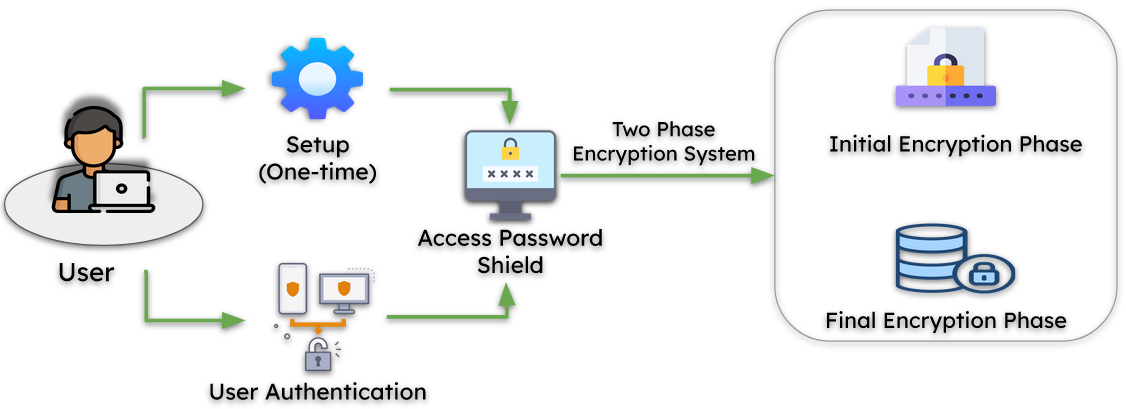
\includegraphics[scale=0.2]{image/method.png}}
\caption{Write proper title of the figure.}
\label{fig1}
\end{figure}

\subsection{Proposed Framework}
Write The Proposed Framework in chapter3.tex

\subsection{Data Set Analysis / Software Project Requirement}
Write the Data Set in chapter3.tex

\begin{table}[htbp]
\caption{Dataset Classes}
\begin{center}
\begin{tabularx}{0.5\textwidth} { 
  | >{\centering\arraybackslash}X 
  | >{\centering\arraybackslash}X 
  | }
\hline
\textbf{-} & \textbf{-}\\
\hline
- & -\\
\hline
- & -\\
\hline
- & -\\
\hline
\end{tabularx}
\label{tab1}
\end{center}
\end{table}

\subsubsection{Subsubsection-1 if necessary}
Write Data Collection \& Prepossessing in chapter3.tex. Write Feature Selection in chapter3.tex

\subsubsection{Subsubsection-2 if necessary}




\subsection{Algorithm/ Model Analysis}
Write the Algorithm in chapter3.tex

\subsection{Explanation of Different Modules}
[if necessary write this segment]
\\
\\
\subsection*{Summary}
Write a Summary passage in chapter3.tex

\clearpage


\cleardoublepage
\begin{center}
    \section*{\fontsize{20}{20}\selectfont Chapter 4}
\end{center}
\vspace{10mm}

\section{Implementation and Result Analysis}
Write an Introductory passage on this topics here in chapter4.tex

\subsection{Environment Setup}
Write Environment Setup in chapter4.tex

\subsection{Data Preprocessing}
Write Data Preprocessing all steps here in chapter4.tex

\subsection{Model Implementation}
Write on Model Implementation here in chapter4.tex

\subsection{Evaluation Metrics}
Write Evaluation Metrics in chapter4.tex

\subsection{Performance Analysis}
Write Performance Analysis in chapter4.tex

\subsection{Key Findings and Discussions}
Write Key Findings and Discussion in chapter4.tex

\subsection{Comparison with State of the Art Model}
Write a Comparison with the State of Art Model in chapter4.tex
\\
\\
\subsection*{Summary}
Write a Summary passage on this chapter here chapter4.tex
\cleardoublepage
\begin{center}
    \section*{\fontsize{20}{20}\selectfont Chapter 5}
\end{center}
\vspace{10mm}

\section{Standards, Constraints, and  Milestones}

Write an Introductory passage of Standards, Constraints, and  Milestones in starting of chapter5.tex

\subsection{Sustainability Standards}
Write Standards in chapter5.tex

\subsection{Impacts on Society }
Write Impacts on Society in chapter5.tex

\subsection{Ethics}
Write Ethics in chapter5.tex

\subsection{Challenges}
Write Challenges in chapter5.tex

\subsection{Constraints}
Write different Constraints like Design constraints, Component Constraints, and Budget constraints in chapter5.tex

\subsection{Timeline and Gantt Chart}
Write Timeline and Gantt Chart in chapter5.tex
\\
\\
\subsection*{Summary}
Write a Summary passage of Standards, Constraints, and  Milestones in end of  chapter5.tex
\cleardoublepage
\begin{center}
    \section*{\fontsize{20}{20}\selectfont Chapter 6}
\end{center}
\vspace{10mm}

\section{Conclusion}
Write the conclusion passage in chapter6.tex

\subsection{Limitations}
Write about Limitations of your work chapter6.tex

\subsection{Future Works and Direction}
Write Future Works and Direction in chapter6.tex
\cleardoublepage



\printbibliography[heading=bibintoc,title={References}]

%%%%%%%%%%%%%%%%%%%%%%%%%%%%%%%%%%%%%%%%%%%%%%%%%%%%%%
% ANNEXURES
%%%%%%%%%%%%%%%%%%%%%%%%%%%%%%%%%%%%%%%%%%%%%%%%%%%%%%

\clearpage
\appendix
\phantomsection
\addcontentsline{toc}{section}{ANNEXURE--I}
%=================== ANNEXURE-I ===================%
\thispagestyle{plain}

\vspace*{\fill}
\begin{center}
    {\Huge\bfseries ANNEXURE--I}\\[1cm]
    {\Large iThenticate: Overall Similarity Score}
\end{center}
\vspace*{\fill}

\clearpage
\thispagestyle{plain}

\begin{center}
    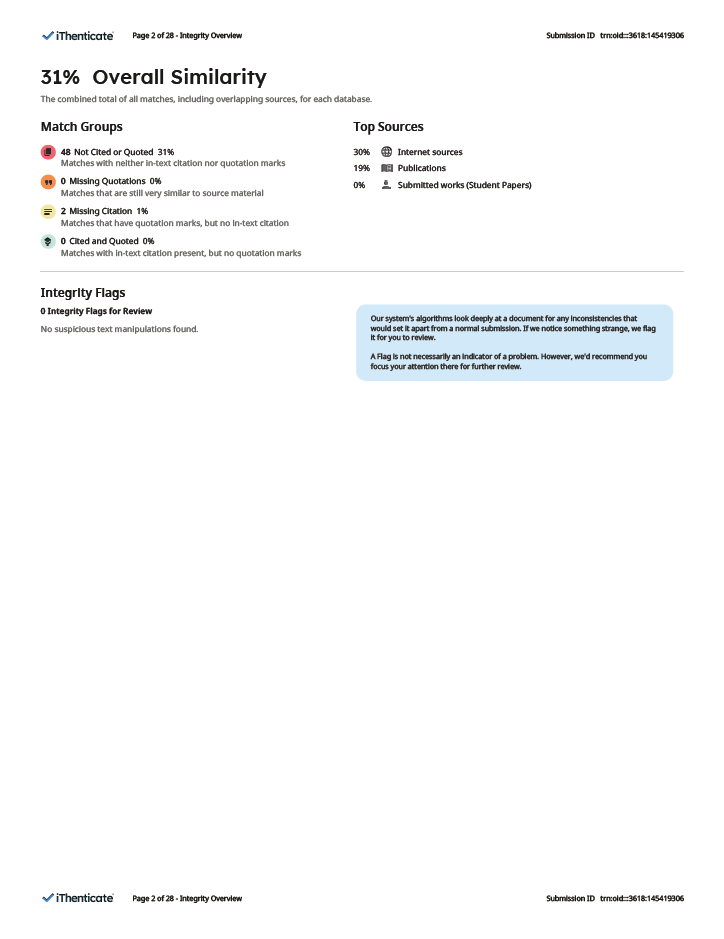
\includegraphics[
        width=\textwidth,
        height=0.95\textheight,
        keepaspectratio
    ]{Similarity Score.png}
\end{center}

\clearpage
\phantomsection
\addcontentsline{toc}{section}{ANNEXURE--II}

%=================== ANNEXURE-II ===================%
\thispagestyle{plain}

\vspace*{\fill}
\begin{center}
    {\Huge\bfseries ANNEXURE--II}\\[1cm]
    {\Large iThenticate: AI Writing Report}
\end{center}
\vspace*{\fill}

\clearpage
\thispagestyle{plain}

\begin{center}
    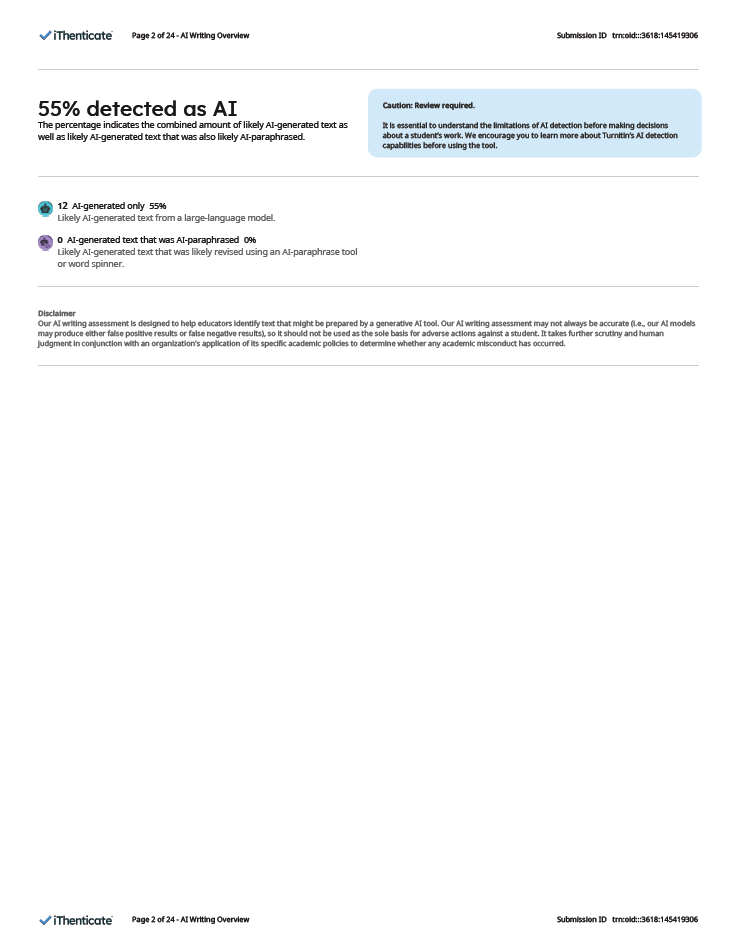
\includegraphics[
        width=\textwidth,
        height=0.95\textheight,
        keepaspectratio
    ]{AI Report.png}
\end{center}

\end{document}